\documentclass[border=4pt]{standalone}
\usepackage{tikz}
\usetikzlibrary{arrows.meta,positioning,shapes.geometric}

\begin{document}
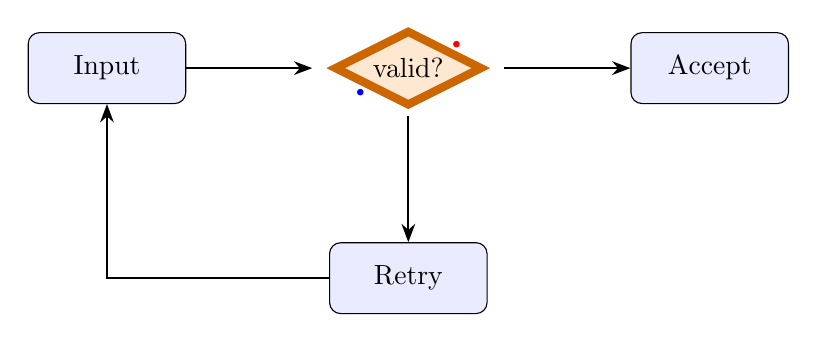
\begin{tikzpicture}[
  >=Stealth,
  node distance=16mm,
  process/.style={draw,rounded corners,minimum width=20mm,minimum height=9mm,fill=blue!8},
  decision/.style={diamond,aspect=2,draw=orange!80!black,line width=3pt,
    fill=orange!18,inner xsep=5pt,inner ysep=2pt,outer xsep=6pt,outer ysep=3pt,
    align=center},
  flow/.style={->,thick}
]
  \node[process] (input) {Input};
  \node[decision,right=of input] (check) {valid?};
  \node[process,right=of check] (accept) {Accept};
  \node[process,below=of check] (retry) {Retry};

  \draw[flow] (input) -- (check);
  \draw[flow] (check) -- (accept);
  \draw[flow] (check.south) -- (retry);
  \draw[flow] (retry.west) -| (input.south);
  \fill[red] (check.north east) circle (1.2pt);
  \fill[blue] (check.south west) circle (1.2pt);
\end{tikzpicture}
\end{document}
